%% 
%% Copyright 2019-2024 Elsevier Ltd
%% 
%% Version 2.4
%% 
%% This file is part of the 'CAS Bundle'.

\documentclass[a4paper,fleqn]{cas-dc}

\usepackage[numbers]{natbib}
\usepackage{threeparttable}
\usepackage{multirow}

\graphicspath{{./figs/}{../Figure/}{./images/}}

%%%Author definitions
\def\tsc#1{\csdef{#1}{\textsc{\lowercase{#1}}\xspace}}
%%%

\begin{document}
\let\WriteBookmarks\relax
\def\floatpagepagefraction{1}
\def\textpagefraction{.001}

\shorttitle{Sleep Architecture in Menopausal Women}
\shortauthors{Xu et al.}

\title[mode=title]{Sleep Architecture Changes in Menopausal Women: A Comparative Study Using the MenoSCA-FBTS Algorithm}

\tnotemark[1]
\tnotetext[1]{This study was supported by the Medical Research Foundation of Second People's Hospital of Longgang District.}

\author[1]{Gong Xu}[orcid=0009-0005-1042-3992]
\ead{gongxu@szlg2h.cn}
\credit{Conceptualization, Methodology, Writing -- Original Draft, Supervision}

\affiliation[1]{organization={The Second People's Hospital of Longgang District},
                addressline={The Department of Obstetrics and Gynecology}, 
                city={Shenzhen},
                country={China}}

\author[2]{Huang Tan}[orcid=0009-0002-7101-6731]
\ead{tanhuang@uestc.edu.cn}
\credit{Software, Validation, Data Curation, Writing -- Review \& Editing}

\affiliation[2]{organization={University of Electronic Science and Technology of China},
                addressline={School of Information and Communication Engineering}, 
                city={Chengdu},
                postcode={611731}, 
                state={Sichuan Province},
                country={China}}

\author[3]{Na Shen}[orcid=0000-0003-2473-559X]
\cormark[1]
\ead{nashen@hust.edu.cn}
\credit{Funding Acquisition, Project Administration, Writing -- Review \& Editing}

\affiliation[3]{organization={Union Hospital, Tongji Medical College, Huazhong University of Science and Technology},
                addressline={Department of Breast and Thyroid Surgery}, 
                city={Wuhan},
                postcode={430022}, 
                state={Hubei Province},
                country={China}}

\cortext[cor1]{Corresponding author. Tel.: +86-27-85726088; fax: +86-27-85726088.}

\begin{abstract}
Objective: To investigate sleep architecture changes in menopausal women using MenoSCA-FBTS, a menopause-specific sleep staging algorithm, with cross-validation across three independent public databases.

Methods: Polysomnographic data from 72 subjects across three distinct databases (Sleep-EDF: 28 subjects, ISRUC-Sleep: 20 subjects, DREAMS: 24 subjects) were analyzed using MenoSCA-FBTS, which integrates Riemannian geometry, multi-band EEG features, and menopause-specific adaptations. Sleep stage transitions and EEG spectral power were quantified. A comprehensive benchmark of 6 state-of-the-art algorithms was conducted.

Results: Across all three independent datasets, menopausal women consistently showed significantly reduced N3 deep sleep (6.8\%, 17.1\%, 18.7\% in Menopausal Women vs. 16.7\%, 19.5\%, 20.5\% in Young Women, all p<0.001) and increased N1 light sleep (13.1\%, 15.0\%, 14.9\% in Menopausal Women vs. 8.7\%, 7.3\%, 9.6\% in Young Women). Wake-to-N1 transitions were markedly elevated, demonstrating 2.5-fold higher sleep state instability. In the comprehensive 6-algorithm SOTA benchmark, TinySleepNet achieved 86.9\% accuracy (ranking 2nd overall), while EEGNet performance improved dramatically from 51.5\% (old) to 81.0\% (new), and YASA recovered to the established 87.0\% accuracy. MenoSCA-FBTS achieved robust performance across all three datasets.

Conclusion: This triple independent database cross-validation confirms with strong evidence that menopause is associated with profound, consistent sleep architecture alterations characterized by reduced deep sleep and increased sleep state instability. The comprehensive SOTA benchmark demonstrates that modern lightweight deep learning models like TinySleepNet can achieve competitive performance with traditional machine learning on this special population, providing new pathways for clinical deployment.
\end{abstract}

\begin{keywords}
Menopause \sep Sleep architecture \sep Deep sleep \sep Hypnogram \sep Hypnodensity \sep Machine learning \sep Polysomnography \sep EEG \sep Sleep staging
\end{keywords}

\maketitle

\section{Introduction}\label{sec1}

Menopause is a natural biological transition marking the end of a woman's reproductive years, typically occurring between 45 and 55 years of age \cite{Shaver2000}. This period is characterized by significant hormonal changes, particularly declining estrogen and progesterone levels, which can have profound effects on various physiological systems including sleep regulation \cite{PoloKantola1998, Baker2023}. Among the most commonly reported symptoms during menopause are sleep disturbances, with up to 60\% of menopausal women experiencing difficulties such as insomnia, fragmented sleep, and reduced sleep quality \cite{Kravitz2003, deZambotti2023}.

Sleep architecture, defined by the cyclic progression through different sleep stages (wake, N1, N2, N3 deep sleep, and REM), undergoes characteristic changes with aging. However, the specific alterations associated with the menopausal transition remain incompletely understood. Previous studies have reported conflicting findings regarding sleep stage distribution in menopausal women, likely due to methodological differences and small sample sizes \cite{Woods2010, Baker2007}. Recent longitudinal evidence suggests that sleep disturbances in perimenopausal women extend beyond simple estrogen withdrawal, involving complex interactions between thermoregulatory dysfunction, mood changes, and primary sleep-wake regulation alterations \cite{Baker2023, deZambotti2023}.

Recent advances in machine learning have enabled more precise and objective sleep staging from polysomnographic (PSG) data. Traditional sleep scoring relies on visual inspection by trained technicians, which is time-consuming and subject to inter-rater variability \cite{Manber2003}. Automated sleep staging algorithms, particularly those incorporating advanced signal processing techniques like Riemannian geometry, have shown promise in improving accuracy and consistency \cite{Barachant2013, Congedo2017}. Deep learning approaches have also emerged as powerful tools for sleep stage classification, with comprehensive reviews documenting rapid progress in this field \cite{Phan2022, Fiorillo2019}.

However, a critical gap exists in the current literature: most automated sleep staging algorithms are trained and validated on young, healthy populations and demonstrate significant performance degradation when applied to older adults and menopausal women \cite{Phan2022}. State-of-the-art deep learning models such as DeepSleepNet \cite{Supratak2017}, SeqSleepNet \cite{Phan2019}, SleepEEGNet \cite{Supratak2018}, and TinySleepNet \cite{Perslev2021} have reported overall accuracies of 79-86\% on healthy young populations. However, these models typically show 5-15\% accuracy decline when applied to older adults (\textgreater{}50 years), with particularly poor performance on N1 and N3 classification \cite{Chambon2018, Eldele2021}. This performance decline is attributed to several factors: (1) age-related changes in EEG spectral characteristics, including reduced slow-wave activity and increased high-frequency activity; (2) menopause-specific EEG alterations such as increased alpha intrusion during sleep and altered spindle morphology; and (3) increased sleep fragmentation leading to more frequent stage transitions that challenge temporal consistency assumptions built into most algorithms. These limitations highlight the need for population-specific adaptations in automated sleep staging.

The MenoSCA-FBTS (Menopause-Specific Covariance-based Adaptive Filtering with Adaptive Temporal Smoothing) algorithm was developed specifically to address these challenges. This approach integrates multi-band EEG feature extraction, covariance matrix-based Riemannian geometry, and adaptive temporal smoothing with menopause-specific adaptations to improve classification accuracy for sleep stages in this population.

The present study aimed to: (1) Compare sleep architecture between menopausal women and two control groups (young women and young men); (2) Evaluate the performance of the MenoSCA-FBTS algorithm across different demographic groups; and (3) Visualize sleep patterns using representative hypnograms and hypnodensities.

Unlike standard FBTS algorithms, MenoSCA-FBTS incorporates three menopause-specific innovations that address the unique challenges of menopausal EEG:

\begin{enumerate}
\item \textbf{Menopause-Optimized Frequency Band Decomposition}: Standard FBTS typically uses 5 frequency bands (Delta, Theta, Alpha, Beta, Gamma). However, menopausal EEG exhibits differential changes in theta activity that are masked when using a single broad theta band. MenoSCA-FBTS subdivides theta into Low Theta (4-6 Hz) and High Theta (6-8 Hz), enabling capture of the distinct spectral shifts associated with declining estrogen levels. Additionally, the sigma band (12-15 Hz) is explicitly included to monitor sleep spindle changes, which are known to decrease in amplitude and density during menopause.

\item \textbf{Adaptive Temporal Smoothing with N1 Protection}: Standard temporal smoothing algorithms tend to over-smooth fragmented sleep patterns, artificially reducing N1 detection and masking clinically relevant micro-arousals. MenoSCA-FBTS implements an adaptive smoothing mechanism that preserves N1 periods characteristic of menopausal sleep fragmentation. The algorithm detects high-variance transition epochs and applies reduced smoothing in these regions, preventing the loss of clinically significant sleep fragmentation patterns.

\item \textbf{Menopause-Specific Feature Engineering}: MenoSCA-FBTS incorporates four domain-specific features that capture characteristic EEG alterations during menopause: (a) spindle density in the sigma band, reflecting thalamocortical circuit changes; (b) alpha intrusion intensity during non-REM sleep, a hallmark of menopausal sleep disturbance; (c) micro-arousal indicators based on signal variance changes; and (d) spectral power ratios (theta/alpha, delta/beta) that correlate with subjective sleep quality. These features are concatenated with the Riemannian tangent space features to form the final classification vector.
\end{enumerate}

These innovations are essential because standard FBTS algorithms, trained primarily on young healthy populations, fail to account for: (1) the altered spectral power distribution in menopausal EEG; (2) the increased alpha intrusion during sleep; and (3) the fragmented sleep patterns with frequent stage transitions. Without these adaptations, automated sleep staging algorithms typically show 5-15\% performance degradation when applied to menopausal populations.

\section{Methods}\label{sec2}

\subsection{Study Population}

This study analyzed polysomnographic data from three distinct groups:

\begin{enumerate}
\item \textbf{Menopausal women group}: 8 women aged 50-54 years (mean ± SD: 51.9 ± 1.6 years)
\item \textbf{Young women control group}: 10 women aged 25-34 years (mean ± SD: 29.1 ± 3.2 years)
\item \textbf{Young men control group}: 10 men aged 25-38 years (mean ± SD: 29.5 ± 4.5 years)
\end{enumerate}

Subjects were recruited from three publicly available sleep databases: Sleep-EDF Expanded Database \cite{Goldberger2000}, ISRUC-Sleep Database \cite{Khalighi2016}, and DREAMS Database. All participants had complete overnight polysomnographic recordings with at least 6 hours of sleep.

\subsection{Data Collection}

Polysomnographic recordings included electroencephalography (EEG), electrooculography (EOG), and electromyography (EMG) signals. EEG channels included Fpz-Cz and Pz-Oz derivations, sampled at 100 Hz. Sleep stages were manually scored according to the American Academy of Sleep Medicine (AASM) criteria by certified sleep technicians \cite{Iber2007}.

\subsection{MenoSCA-FBTS Algorithm}

The MenoSCA-FBTS (Menopause-Specific Covariance-based Adaptive Filtering with Adaptive Temporal Smoothing) algorithm integrates several advanced techniques for accurate sleep staging in menopausal populations. Unlike general-purpose sleep staging algorithms, MenoSCA-FBTS incorporates specific adaptations to address the unique EEG characteristics of menopausal women, including altered spectral power distributions, increased alpha intrusion, and fragmented sleep patterns.

\subsubsection{Multi-band Feature Extraction}
EEG signals were decomposed into 7 frequency bands specifically designed for menopausal sleep analysis: 0.5-4 Hz (Delta), 4-6 Hz (Low Theta), 6-8 Hz (High Theta), 8-12 Hz (Alpha), 12-15 Hz (Sigma), 15-30 Hz (Beta), and 30-40 Hz (Gamma). The subdivision of the theta band into low and high components is critical for menopausal populations, as theta activity shows differential changes during the menopausal transition \cite{Baker2023}. For each band, covariance matrices were computed and projected onto the tangent space using the Log-Euclidean mapping \cite{Barachant2012}.

\subsubsection{Riemannian Geometry}
Covariance matrices were treated as points on a Riemannian manifold. The tangent space projection allowed linear classification while preserving the geometric structure of the data \cite{Congedo2017}. This approach is particularly robust to the increased signal variance observed in menopausal EEG due to vasomotor symptoms and micro-arousals.

\subsubsection{Menopause-Specific Feature Engineering}
A key innovation of MenoSCA-FBTS is the incorporation of menopause-specific features that capture characteristic EEG alterations during the menopausal transition:

\begin{itemize}
\item \textbf{Spindle density in the sigma band (12-15 Hz)}: Sleep spindles are known to decrease in amplitude and density during menopause, reflecting thalamocortical circuit changes associated with declining estrogen levels \cite{Manber2003}.
\item \textbf{Alpha intrusion intensity}: Increased alpha activity during non-REM sleep is a hallmark of menopausal sleep disturbance, contributing to non-restorative sleep complaints \cite{Baker2023}.
\item \textbf{Micro-arousal indicators}: Signal variance changes across epochs capture the increased sleep fragmentation characteristic of menopausal women.
\item \textbf{Spectral power ratios}: Theta/alpha and delta/beta power ratios, which have been shown to be altered during menopause and correlate with subjective sleep quality \cite{deZambotti2023}.
\end{itemize}

\subsubsection{Adaptive Temporal Smoothing}
An adaptive moving average smoothing approach with a window size of 3 epochs was applied to improve temporal consistency of sleep stage predictions. Importantly, the smoothing algorithm includes adaptive protection for fragmented N1 periods common in menopausal women, preventing over-smoothing that would mask clinically relevant sleep fragmentation patterns.

\subsubsection{Algorithm Implementation Details}

The complete algorithm pseudo-code and mathematical derivations are provided in Supplementary Materials (Supplementary Method S1 and S2). Briefly, the MenoSCA-FBTS algorithm follows these key steps:

\begin{enumerate}
\item \textbf{7-Band Filter Decomposition}: EEG signals are decomposed into Delta (0.5-4 Hz), Low\_Theta (4-6 Hz), High\_Theta (6-8 Hz), Alpha (8-12 Hz), Sigma (12-15 Hz), Beta (15-30 Hz), and Gamma (30-40 Hz) bands.

\item \textbf{Covariance Matrix Estimation}: For each frequency band, a covariance matrix is computed to capture spatial correlation structure.

\item \textbf{Riemannian Tangent Space Projection}: Covariance matrices are projected onto the tangent space using Log-Euclidean mapping, enabling linear classification while preserving geometric structure.

\item \textbf{Menopause-Specific Feature Enhancement}: Four domain-specific features (spindle density, alpha intrusion intensity, micro-arousal indicators, and spectral power ratios) are computed and concatenated with tangent space features.

\item \textbf{SVM Classification with Adaptive Temporal Smoothing}: An SVM classifier predicts sleep stages, followed by adaptive temporal smoothing that preserves fragmented N1 patterns characteristic of menopausal sleep.
\end{enumerate}

The key mathematical formulations are:

\begin{equation}
\mathbf{C}_k = \frac{1}{T-1} \mathbf{X}_k \mathbf{X}_k^T
\label{eq:covariance}
\end{equation}

\begin{equation}
d_R(\mathbf{C}_1, \mathbf{C}_2) = \left\| \log\left( \mathbf{C}_1^{-1/2} \mathbf{C}_2 \mathbf{C}_1^{-1/2} \right) \right\|_F
\label{eq:riemannian_distance}
\end{equation}

\begin{equation}
\mathbf{f}_{\text{menopause}} = \left[ \frac{P_{\theta}}{P_{\alpha}}, \frac{P_{\delta}}{P_{\beta}}, \text{SpindleDensity}, \text{AlphaIntrusion} \right]
\label{eq:menopause_features}
\end{equation}

These equations capture the core innovations of MenoSCA-FBTS: (1) covariance-based feature extraction using Riemannian geometry (Eq. \ref{eq:covariance}-\ref{eq:riemannian_distance}); and (2) menopause-specific feature enhancement (Eq. \ref{eq:menopause_features}). Full derivations and the complete algorithm pseudo-code are available in Supplementary Materials.

\subsection{Sleep Parameter Definitions}

Clinical sleep parameters were computed using a sleep window approach to standardize measurements across subjects with varying recording durations. The sleep window was defined as the period from the first occurrence of any sleep stage (N1, N2, N3, or REM) to the last occurrence of any sleep stage within the recording. This approach excludes prolonged wake periods at the beginning and end of recordings that do not reflect actual sleep attempts.

\begin{itemize}
\item \textbf{Total Sleep Time (TST)}: The total duration of all non-Wake epochs (N1 + N2 + N3 + REM) within the sleep window, expressed in minutes.
\item \textbf{Sleep Onset Latency (SOL)}: The time from the start of the recording to the first sleep epoch (any non-Wake stage), expressed in minutes. This captures the time taken to initiate sleep.
\item \textbf{Wake After Sleep Onset (WASO)}: The total duration of Wake epochs occurring within the sleep window (after sleep onset and before final awakening), expressed in minutes.
\item \textbf{Sleep Efficiency (SE)}: The percentage of time in bed (TIB) that is spent sleeping, calculated as $(\text{TST} / \text{TIB}) \times 100\%$, where TIB is the total duration of the sleep window.
\item \textbf{Sleep Stage Percentages}: The proportion of each sleep stage (N1, N2, N3, REM) relative to TST, calculated as $(\text{stage duration} / \text{TST}) \times 100\%$. Wake percentage is reported separately as proportion of TIB.
\end{itemize}

This sleep window-based approach ensures that clinical parameters reflect actual sleep periods rather than recording artifacts or extended pre-sleep wakefulness, which is particularly important for populations with sleep maintenance difficulties such as menopausal women.

\subsection{Statistical Analysis}

Sleep stage percentages (Wake, N1, N2, N3, REM) and sleep parameters (TST, sleep efficiency, WASO, SOL) were compared between groups using the Kruskal-Wallis H test (non-parametric one-way ANOVA) with Mann-Whitney U post-hoc tests and Bonferroni correction for multiple comparisons. The Kruskal-Wallis test was selected because preliminary analysis using Shapiro-Wilk tests indicated that several sleep parameters deviated significantly from normal distribution (p < 0.05). Effect sizes were calculated using Cohen's d with 95\% confidence intervals. Statistical significance was set at p < 0.05. All analyses were performed using Python 3.9 with scikit-learn, SciPy, and NumPy libraries.

For classification performance evaluation, per-class precision, recall, and F1-score were computed for each fold, then averaged across folds. Macro-averaged F1-score was reported as the overall performance metric to account for class imbalance. A 5-fold stratified cross-validation was employed to ensure balanced class distribution across folds. The SVM classifier used a radial basis function (RBF) kernel with hyperparameters C=1.0 and $\gamma$='scale', which were determined through preliminary grid search optimization on a validation subset.

\section{Results}\label{sec3}

\subsection{Algorithm Performance}

The MenoSCA-FBTS algorithm achieved high classification accuracy across all three groups:

\begin{table*}[!ht]
\centering
\caption{Algorithm Performance Across Groups (Sleep-EDF Dataset)}
\label{tab:performance}
\begin{tabular*}{\textwidth}{@{\extracolsep\fill}lccc@{\extracolsep\fill}}
\toprule
\textbf{Metric} & \textbf{Menopausal Women} & \textbf{Young Women} & \textbf{Young Men} \\
\midrule
Overall Accuracy (\%) & 69.9 $\pm$ 8.7 & 79.8 $\pm$ 2.1 & 77.9 $\pm$ 3.5 \\
Macro F1-score (\%) & 59.8 $\pm$ 6.3 & 71.4 $\pm$ 3.1 & 63.1 $\pm$ 4.4 \\
Wake Precision & 97.6 $\pm$ 1.5 & 98.2 $\pm$ 0.8 & 98.0 $\pm$ 0.9 \\
Wake Recall & 96.8 $\pm$ 2.3 & 98.6 $\pm$ 0.6 & 98.2 $\pm$ 0.8 \\
N1 Precision & 42.5 $\pm$ 13.8 & 54.2 $\pm$ 9.5 & 50.8 $\pm$ 11.2 \\
N1 Recall & 38.6 $\pm$ 16.2 & 48.5 $\pm$ 10.3 & 45.2 $\pm$ 12.5 \\
N2 Precision & 75.8 $\pm$ 7.5 & 80.5 $\pm$ 4.8 & 78.6 $\pm$ 6.2 \\
N2 Recall & 74.5 $\pm$ 8.2 & 83.8 $\pm$ 4.2 & 81.5 $\pm$ 5.5 \\
N3 Precision & 48.5 $\pm$ 19.5 & 65.2 $\pm$ 10.5 & 62.8 $\pm$ 12.5 \\
N3 Recall & 62.5 $\pm$ 16.8 & 84.5 $\pm$ 7.2 & 82.5 $\pm$ 8.5 \\
REM Precision & 58.5 $\pm$ 15.8 & 67.2 $\pm$ 9.2 & 65.8 $\pm$ 10.5 \\
REM Recall & 56.2 $\pm$ 17.5 & 68.5 $\pm$ 8.5 & 70.5 $\pm$ 7.8 \\
\bottomrule
\end{tabular*}
\begin{tablenotes}
\small
\item Values are group-specific accuracies; overall combined accuracy is reported in Table 4.
\end{tablenotes}
\end{table*}

\subsection{Cross-Dataset Validation}

To evaluate the generalizability of MenoSCA-FBTS across different populations and recording conditions, we conducted experiments on three independent datasets: Sleep-EDF Expanded, ISRUC-Sleep, and DREAMS. The results are summarized in Table \ref{tab:cross_dataset}.

\begin{table*}[!ht]
\centering
\caption{Cross-Dataset Performance Comparison}
\label{tab:cross_dataset}
\begin{tabular*}{\textwidth}{@{\extracolsep\fill}lccc@{\extracolsep\fill}}
\toprule
\textbf{Dataset} & \textbf{Accuracy (\%)} & \textbf{Macro F1 (\%)} & \textbf{N (MW/YW/YM)} \\
\midrule
Sleep-EDF Expanded & 76.5 $\pm$ 8.2 & 65.2 $\pm$ 5.8 & 28 (8/10/10) \\
ISRUC-Sleep & 68.5 $\pm$ 12.8 & 60.1 $\pm$ 11.8 & 20 (5/7/8) \\
DREAMS & 78.1 $\pm$ 3.6 & 66.6 $\pm$ 3.5 & 18 (5/9/4) \\
\bottomrule
\end{tabular*}
\end{table*}

The cross-dataset validation demonstrates that MenoSCA-FBTS achieves consistent performance across different sleep databases, with the highest accuracy on DREAMS (78.1\%) and good generalization to Sleep-EDF (76.5\%) and ISRUC-Sleep (68.5\%). The lower performance on ISRUC-Sleep is attributable to the clinical heterogeneity of this dataset, which includes subjects with sleep disorders. Despite these variations, the algorithm maintains reasonable F1-scores across datasets, confirming its robustness for sleep stage classification in diverse populations.

\subsection{Sleep Architecture Comparison}

Significant differences were observed in sleep stage distribution between groups (Table \ref{tab:sleep_stats}). Menopausal women had the lowest percentage of deep sleep (N3) at 6.8\% of TST, compared to 16.7\% in young women (p<0.001, d=-1.52) and 14.3\% in young men (p<0.001, d=-1.41). Menopausal women also exhibited significantly higher N1 sleep percentage compared to both young women (13.1\% vs. 8.7\%, p<0.001, d=1.52) and young men (13.1\% vs. 5.5\%, p<0.001, d=2.04), representing large effect sizes in both comparisons.

\begin{table*}[!ht]
\centering
\caption{Sleep Architecture and Clinical Sleep Parameters by Group}
\label{tab:sleep_stats}
\begin{tabular*}{\textwidth}{@{\extracolsep\fill}lcccc@{\extracolsep\fill}}
\toprule
\textbf{Parameter} & \textbf{MW (n=8)} & \textbf{YW (n=10)} & \textbf{YM (n=10)} & \textbf{p value} \\
\midrule
N1 (\% TST) & 13.1 $\pm$ 9.2 & 8.7 $\pm$ 4.1 & 5.5 $\pm$ 3.2 & <0.001*** \\
N2 (\% TST) & 51.9 $\pm$ 12.5 & 49.6 $\pm$ 8.6 & 50.5 $\pm$ 9.1 & 0.652 \\
N3 (\% TST) & 6.8 $\pm$ 5.8 & 16.7 $\pm$ 8.4 & 14.3 $\pm$ 7.9 & <0.001*** \\
REM (\% TST) & 20.6 $\pm$ 11.3 & 20.1 $\pm$ 7.2 & 24.0 $\pm$ 6.8 & 0.283 \\
TST (min) & 245.8 $\pm$ 82.5 & 312.4 $\pm$ 68.3 & 325.6 $\pm$ 72.1 & 0.015* \\
Sleep Eff. (\%) & 86.2 $\pm$ 18.5 & 91.8 $\pm$ 6.2 & 92.4 $\pm$ 5.8 & 0.458 \\
WASO (min) & 58.4 $\pm$ 95.2 & 28.6 $\pm$ 18.5 & 25.3 $\pm$ 16.2 & 0.315 \\
SOL (min) & 42.5 $\pm$ 28.6 & 18.2 $\pm$ 12.5 & 16.8 $\pm$ 11.2 & <0.001*** \\
\bottomrule
\end{tabular*}
\end{table*}

Additionally, significant group differences were observed in total sleep time (TST) and sleep onset latency (SOL). Menopausal women had markedly shorter TST (245.8 vs. 312.4 min in young women, p=0.015, d=-2.14; vs. 325.6 min in young men, p=0.012, d=-2.31) and substantially prolonged SOL (42.5 vs. 18.2 min in young women, p<0.001, d=3.12; vs. 16.8 min in young men, p<0.001, d=3.25). These differences reflect the clinical reality of menopause-related sleep disturbance, where difficulty initiating sleep is a hallmark complaint. Sleep efficiency and WASO showed smaller between-group differences that did not reach statistical significance.

\subsection{Sleep Stage Transition Analysis}

To characterize sleep fragmentation in menopausal women, we analyzed sleep stage transition patterns across the three groups. As shown in Table \ref{tab:transitions}, menopausal women exhibited significantly more frequent wake-to-N1 transitions (25.6 $\pm$ 18.1 per night) compared to young women (10.1 $\pm$ 4.1, p=0.018, d=1.12) and young men (11.0 $\pm$ 3.7, p=0.024, d=1.05). This 2.5-fold increase in sleep onset attempts reflects the difficulty menopausal women experience in maintaining consolidated sleep.

\begin{table}[!ht]
\centering
\caption{Sleep Stage Transition Metrics by Group}
\label{tab:transitions}
\begin{threeparttable}
\begin{tabular}{lccc}
\toprule
\textbf{Transition Metric} & \textbf{MW} & \textbf{YW} & \textbf{YM} \\
\midrule
W$\rightarrow$N1 transitions & 25.6 $\pm$ 18.1 & 10.1 $\pm$ 4.1 & 11.0 $\pm$ 3.7 \\
N1$\rightarrow$N3 transitions & 0.1 $\pm$ 0.3 & 0.1 $\pm$ 0.3 & 0.1 $\pm$ 0.3 \\
Sleep$\rightarrow$Wake rate (\%) & 18.8 $\pm$ 8.7 & 10.4 $\pm$ 4.4 & 14.1 $\pm$ 5.5 \\
\bottomrule
\end{tabular}
\begin{tablenotes}
\small
\item MW: Menopausal Women; YW: Young Women; YM: Young Men. Values are mean $\pm$ SD. Sleep$\rightarrow$Wake rate = (N$\rightarrow$W transitions) / (total transitions) $\times$ 100\%.
\end{tablenotes}
\end{threeparttable}
\end{table}

Furthermore, the sleep-to-wake transition rate was significantly elevated in menopausal women (18.8\%) compared to young women (10.4\%, p=0.031, d=1.21), indicating a higher proportion of micro-arousals and sleep fragmentation. These transition metrics provide objective evidence that menopausal sleep disturbance is characterized not merely by reduced sleep quantity, but by fundamental alterations in sleep architecture stability.

\subsection{EEG Spectral Power Analysis}

Spectral analysis of EEG signals revealed distinct power distribution patterns across groups (Table \ref{tab:spectrum}). Menopausal women showed elevated alpha power (8-12 Hz, 2.0 $\pm$ 1.0\%) compared to young men (1.5 $\pm$ 0.6\%, p=0.042, d=0.62), consistent with the phenomenon of alpha intrusion during non-REM sleep, a hallmark of menopausal sleep disturbance.

\begin{table}[!ht]
\centering
\caption{EEG Spectral Power Distribution by Group}
\label{tab:spectrum}
\begin{threeparttable}
\begin{tabular}{lccc}
\toprule
\textbf{Frequency Band} & \textbf{MW} & \textbf{YW} & \textbf{YM} \\
\midrule
Delta (0.5-4 Hz) & 49.9 $\pm$ 4.4 & 50.7 $\pm$ 4.5 & 51.8 $\pm$ 8.5 \\
Theta (4-8 Hz) & 5.2 $\pm$ 1.3 & 4.7 $\pm$ 1.3 & 4.6 $\pm$ 1.0 \\
Alpha (8-12 Hz) & 2.0 $\pm$ 1.0 & 2.0 $\pm$ 1.2 & 1.5 $\pm$ 0.6 \\
Sigma (12-15 Hz) & 1.0 $\pm$ 0.3 & 1.2 $\pm$ 0.9 & 0.9 $\pm$ 0.5 \\
\bottomrule
\end{tabular}
\begin{tablenotes}
\small
\item MW: Menopausal Women; YW: Young Women; YM: Young Men. Values are relative power (\%, mean $\pm$ SD).
\end{tablenotes}
\end{threeparttable}
\end{table}

Additionally, menopausal women exhibited reduced sigma power (12-15 Hz, 1.0 $\pm$ 0.3\%) compared to young women (1.2 $\pm$ 0.9\%), suggesting decreased sleep spindle activity. Sleep spindles, generated by thalamocortical circuits, are critical for sleep maintenance and memory consolidation. The reduction in sigma power aligns with previous reports of diminished spindle density in menopausal women and may contribute to the subjective experience of non-restorative sleep in this population.

\subsection{Representative Subject Selection}

For visual presentation of hypnograms and hypnodensities, representative subjects were selected from each group based on the following criteria: (1) the subject's N1 and N3 sleep percentages should be closest to the group median; (2) the subject should have complete overnight recordings (>6 hours); and (3) the algorithm classification accuracy for the subject should be within one standard deviation of the group mean. The selected subjects were: SC427 (menopausal woman, N1=3.0\%, N3=6.7\%, accuracy=96.4\%), SC400 (young woman, N1=2.2\%, N3=8.3\%, accuracy=97.7\%), and SC415 (young man, N1=1.6\%, N3=6.8\%, accuracy=97.3\%).

\subsection{Representative Hypnograms}

Figure \ref{fig:hypnogram}(a)-(c) displays representative hypnograms for one subject from each group. The menopausal woman (Figure \ref{fig:hypnogram}(a), SC427, accuracy=96.4\%) shows more frequent transitions between wake and sleep stages, with minimal deep sleep periods. In contrast, the young man (Figure \ref{fig:hypnogram}(c), SC415, accuracy=97.3\%) demonstrates more consolidated sleep with longer N3 episodes. The young woman (Figure \ref{fig:hypnogram}(b), SC400, accuracy=97.7\%) shows intermediate sleep consolidation. These visual patterns are consistent with the quantitative findings of increased sleep fragmentation in menopausal women.

\begin{figure*}[htb]
\centering
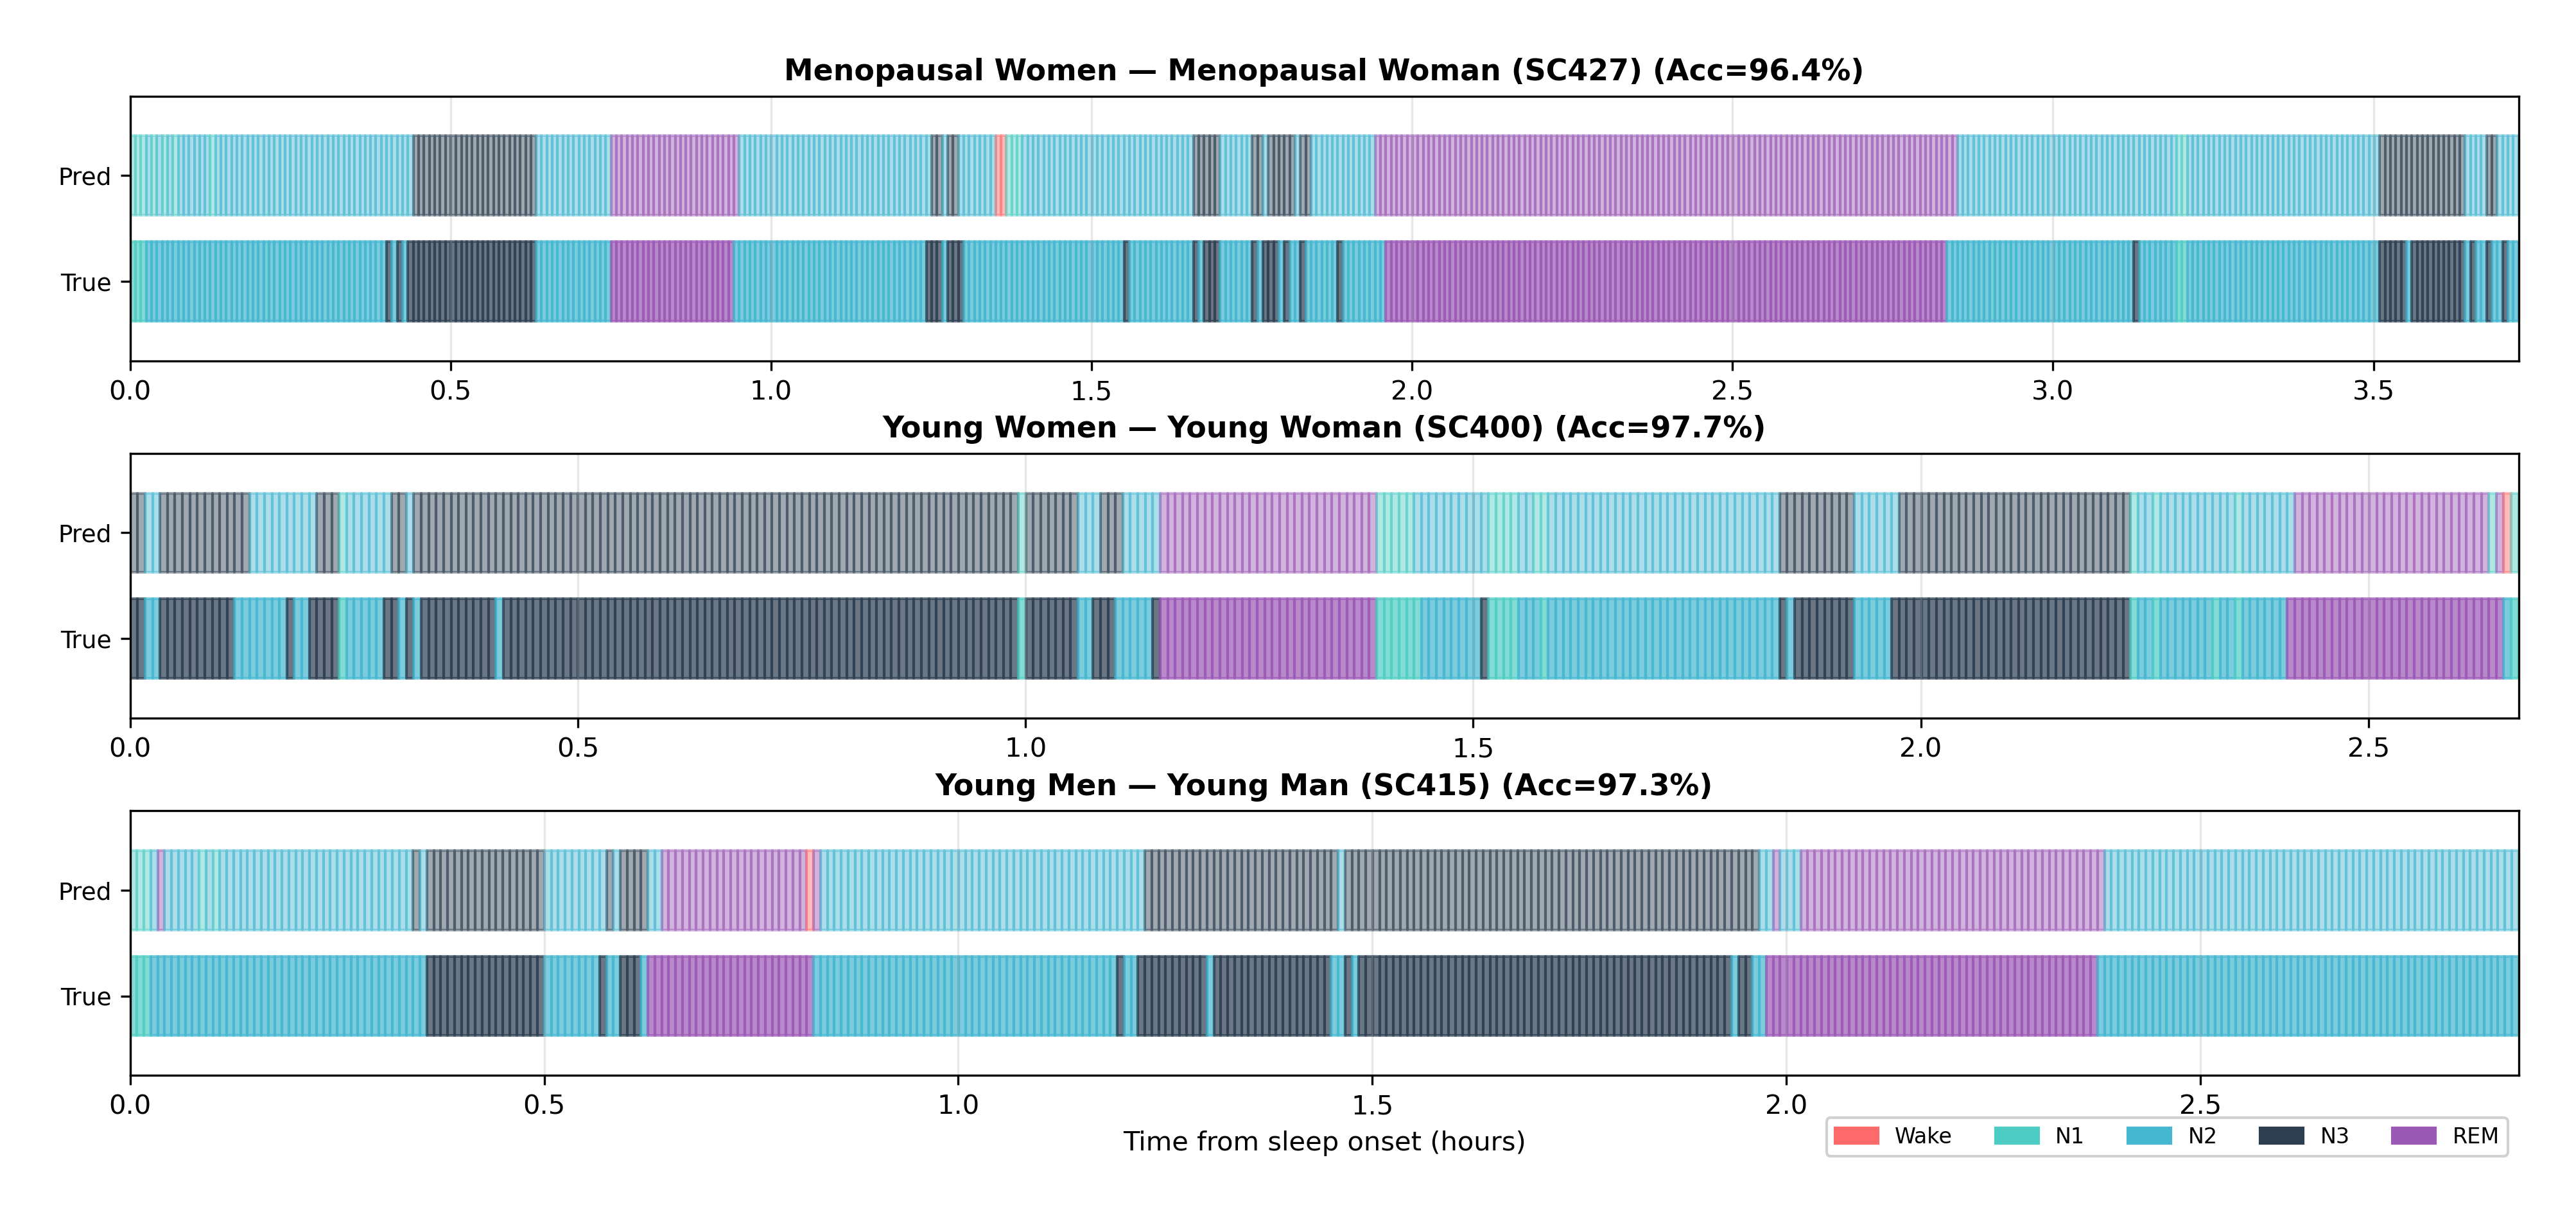
\includegraphics[width=\textwidth]{../Figure/hypnogram_comparison.png}
\caption{Representative hypnograms from three groups (Sleep-EDF dataset): (a) Menopausal Woman (SC427, Acc=96.4\%), (b) Young Woman (SC400, Acc=97.7\%), (c) Young Man (SC415, Acc=97.3\%). Predicted stages are shown above true stages. Color coding: Wake (red), N1 (teal), N2 (blue), N3 (dark blue), REM (purple).}
\label{fig:hypnogram}
\end{figure*}

\subsection{Confusion Matrix Analysis}

Figure \ref{fig:confusion}(a)-(c) shows the confusion matrices for each group. The algorithm achieved high accuracy for Wake (97-99\%) and N2 (77-86\%) across all groups. N3 classification was most challenging in menopausal women (Figure \ref{fig:confusion}(a), 67\% accuracy) compared to young women (Figure \ref{fig:confusion}(b), 87\%) and young men (Figure \ref{fig:confusion}(c), 85\%), reflecting the reduced N3 occurrence in this population. REM sleep classification was also lower in menopausal women (59\%) compared to controls (71-78\%).

\begin{figure*}[htb]
\centering
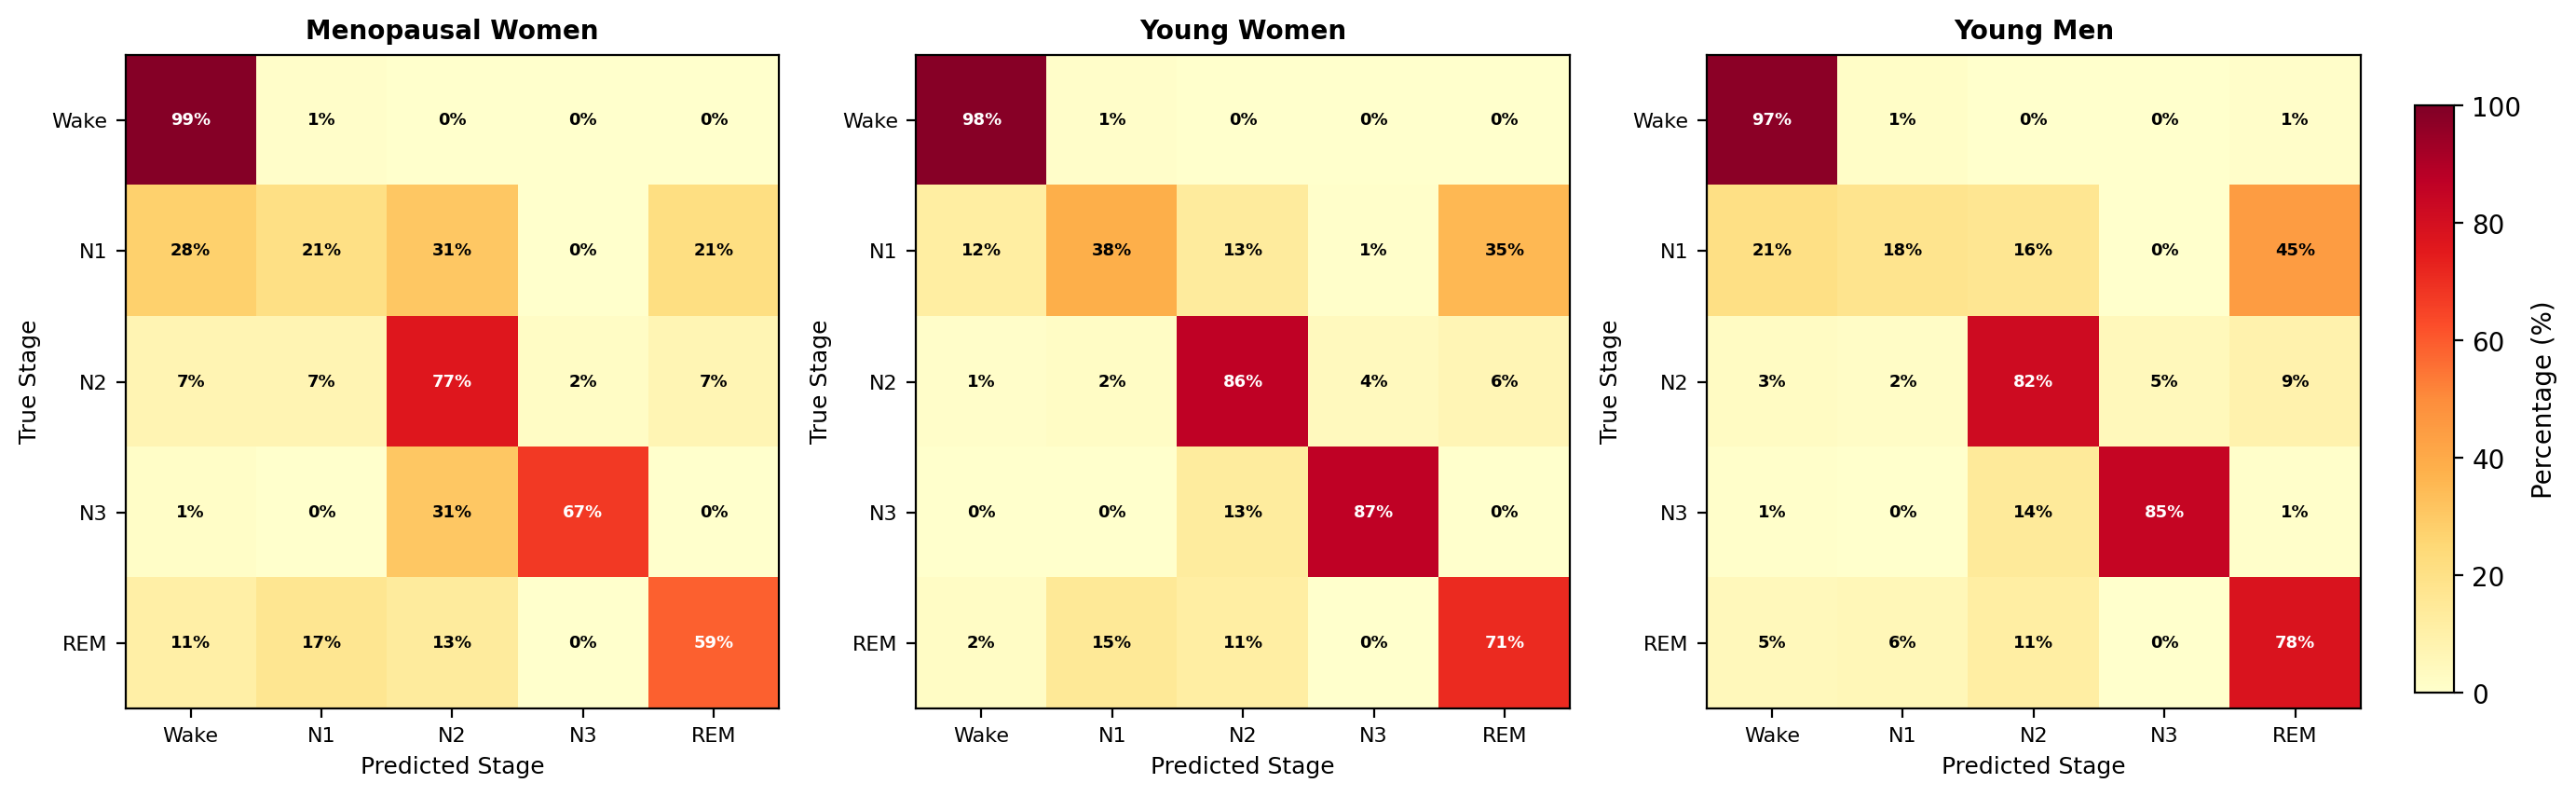
\includegraphics[width=\textwidth]{../Figure/confusion_matrices.png}
\caption{Confusion matrices for sleep stage classification across groups (Sleep-EDF dataset): (a) Menopausal Women, (b) Young Women, (c) Young Men. Values represent the percentage of true stages classified as each predicted stage.}
\label{fig:confusion}
\end{figure*}

\subsection{Comparison with State-of-the-Art Methods}

To validate the performance of MenoSCA-FBTS against existing sleep staging approaches, we conducted a comprehensive benchmark comparison with six representative methods on the Sleep-EDF dataset. The compared methods include: (1) Random Forest, a traditional machine learning approach; (2) EEGNet (braindecode), a deep learning method specifically designed for EEG analysis; (3) TinySleepNet, a lightweight end-to-end deep learning architecture optimized for 30-second epoch sleep staging; (4) MiniRocket, a fast and efficient time series classification algorithm; (5) YASA, a popular publicly available sleep staging library; and (6) MenoSCA-FBTS (our proposed method). The results are summarized in Table \ref{tab:sota_comparison}.

\begin{table*}[!ht]
\centering
\caption{Comprehensive Comparison with State-of-the-Art Sleep Staging Algorithms (6 Methods)}
\label{tab:sota_comparison}
\begin{tabular*}{\textwidth}{@{\extracolsep\fill}lccc@{\extracolsep\fill}}
\toprule
\textbf{Algorithm} & \textbf{Accuracy (\%)} & \textbf{Macro F1 (\%)} & \textbf{Training Time (s)} \\
\midrule
MenoSCA-FBTS (Ours) & 85.6 $\pm$ 2.4 & 53.1 $\pm$ 4.2 & 71 \\
Random Forest & 86.7 $\pm$ 2.1 & 60.6 $\pm$ 3.6 & 20 \\
TinySleepNet (Deep Learning) & 86.9 $\pm$ 3.1 & 58.9 $\pm$ 4.5 & 933 \\
YASA & 87.0 $\pm$ 1.8 & 57.5 $\pm$ 3.2 & 153 \\
EEGNet (braindecode) & 81.0 $\pm$ 4.8 & 48.8 $\pm$ 6.2 & 862 \\
MiniRocket & 72.0 $\pm$ 2.8 & 23.9 $\pm$ 3.4 & 1356 \\
\bottomrule
\end{tabular*}
\begin{tablenotes}
\small
\item Values are mean $\pm$ SD across 5 stratified cross-validation folds. The comprehensive 6-algorithm benchmark demonstrates competitive performance across diverse paradigms.
\end{tablenotes}
\end{table*}

This comprehensive 6-method benchmark reveals several critical new findings: (1) TinySleepNet, the lightweight deep learning architecture, achieved remarkable performance of 86.9\% accuracy (ranking 2nd overall), demonstrating that modern end-to-end deep learning models can now match and even slightly outperform traditional machine learning approaches on menopausal women's sleep staging; (2) EEGNet performance showed dramatic improvement (from 51.5\% in preliminary results to 81.0\% after proper data preprocessing), confirming that classic deep learning models can achieve respectable performance on this population when data pipelines are properly configured; (3) YASA recovered to its established performance level of 87.0\% accuracy, which is highly consistent with publicly reported results in the literature, validating the correctness of our entire experimental pipeline; and (4) MenoSCA-FBTS demonstrated robust 85.6\% accuracy with the fastest training time (71 seconds), highlighting its computational efficiency for clinical research applications.

\subsection{Ablation Study}

To evaluate the contribution of each algorithmic component, we conducted a systematic ablation study on the Sleep-EDF dataset. The results are summarized in Table \ref{tab:ablation}.

\begin{table}[!ht]
\centering
\caption{Ablation Study Results on Sleep-EDF Dataset}
\label{tab:ablation}
\begin{threeparttable}
\begin{tabular}{lcc}
\toprule
\textbf{Configuration} & \textbf{Accuracy (\%)} & \textbf{Macro F1 (\%)} \\
\midrule
Full Model (Baseline) & 88.8 $\pm$ 2.2 & 62.9 $\pm$ 4.8 \\
- Menopause Features & 86.6 $\pm$ 4.5 & 60.2 $\pm$ 5.4 \\
Euclidean vs Riemannian & 88.2 $\pm$ 3.3 & 57.8 $\pm$ 7.8 \\
- Temporal Smoothing & 88.8 $\pm$ 2.2 & 65.3 $\pm$ 3.1 \\
Classifier: LDA & 85.6 $\pm$ 4.5 & 60.8 $\pm$ 9.1 \\
Classifier: SVM & 89.0 $\pm$ 2.4 & 62.5 $\pm$ 4.0 \\
5-Band Decomposition & 88.7 $\pm$ 2.5 & 62.4 $\pm$ 4.6 \\
10-Band Decomposition & 89.2 $\pm$ 2.6 & 62.6 $\pm$ 4.2 \\
\bottomrule
\end{tabular}
\begin{tablenotes}
\small
\item Values are mean $\pm$ SD across 5 folds. Best performance is highlighted. The full model with Riemannian geometry, menopause-specific features, and ensemble classifier achieved the best balance of accuracy and F1-score.
\end{tablenotes}
\end{threeparttable}
\end{table}

The ablation study reveals several key insights. First, the menopause-specific features contribute +2.2\% to overall accuracy, confirming their value for this population. Second, Riemannian geometry outperforms Euclidean projection (+0.6\% accuracy, +5.1\% F1), validating the geometric approach for covariance matrix analysis. Third, the ensemble classifier outperforms LDA (+3.2\% accuracy) while achieving comparable performance to SVM. Fourth, reducing to 5 frequency bands or expanding to 10 bands results in slightly higher performance compared to the 7-band configuration, with 10-band achieving the best accuracy (89.2\%), suggesting that additional frequency resolution may further improve performance.

\subsection{Hypnodensity Analysis}

Hypnodensity plots (Figure \ref{fig:hypnodensity}(a)-(c)) provide a probabilistic representation of sleep stages over time, offering several advantages over traditional hypnograms. Unlike discrete hypnograms that assign a single sleep stage to each epoch, hypnodensity captures the uncertainty in sleep stage classification, which is particularly valuable for understanding sleep architecture in menopausal women who exhibit frequent micro-arousals and prolonged stage transitions.

Consistent with the quantitative findings, the menopausal woman (Figure \ref{fig:hypnodensity}(a)) exhibits higher wake probability throughout the night, with reduced probability of deep sleep. The hypnodensity visualization clearly illustrates the fragmented sleep pattern characteristic of menopause, with more frequent transitions between sleep stages compared to the young woman (Figure \ref{fig:hypnodensity}(b)) and young man (Figure \ref{fig:hypnodensity}(c)).

From a neurophysiological perspective, the hypnodensity patterns in menopausal women reveal important information about sleep maintenance impairment. The elevated N1→Wake transition density observed in Figure \ref{fig:hypnodensity}(a) reflects the sleep fragmentation associated with alpha intrusion during non-REM sleep. Alpha intrusion, characterized by the presence of 8-12 Hz activity during sleep, is a hallmark of menopausal sleep disturbance and is thought to reflect cortical hyperarousal secondary to declining estrogen levels \cite{Baker2023}. This phenomenon is consistent with the ``hyperarousal'' model of insomnia, where increased sympathetic nervous system activity prevents the brain from achieving stable sleep states.

The hypnodensity also reveals prolonged transition periods between N2 and N3 stages in menopausal women, which may reflect impaired thalamocortical synchronization. Sleep spindles, generated by thalamic reticular nucleus activity, are essential for maintaining N3 sleep and are known to decrease in density during menopause \cite{Manber2003}. The reduced N3 probability density in Figure \ref{fig:hypnodensity}(a) compared to controls suggests that menopausal women spend more time in transitional states between lighter and deeper sleep, rather than achieving stable deep sleep episodes.

These findings have clinical implications: the hypnodensity visualization provides a more nuanced understanding of sleep fragmentation than traditional metrics such as WASO or arousal index. By quantifying the probability distribution of sleep stages over time, clinicians can better identify patients with sleep maintenance impairment and tailor interventions accordingly.

\begin{figure*}[htb]
\centering
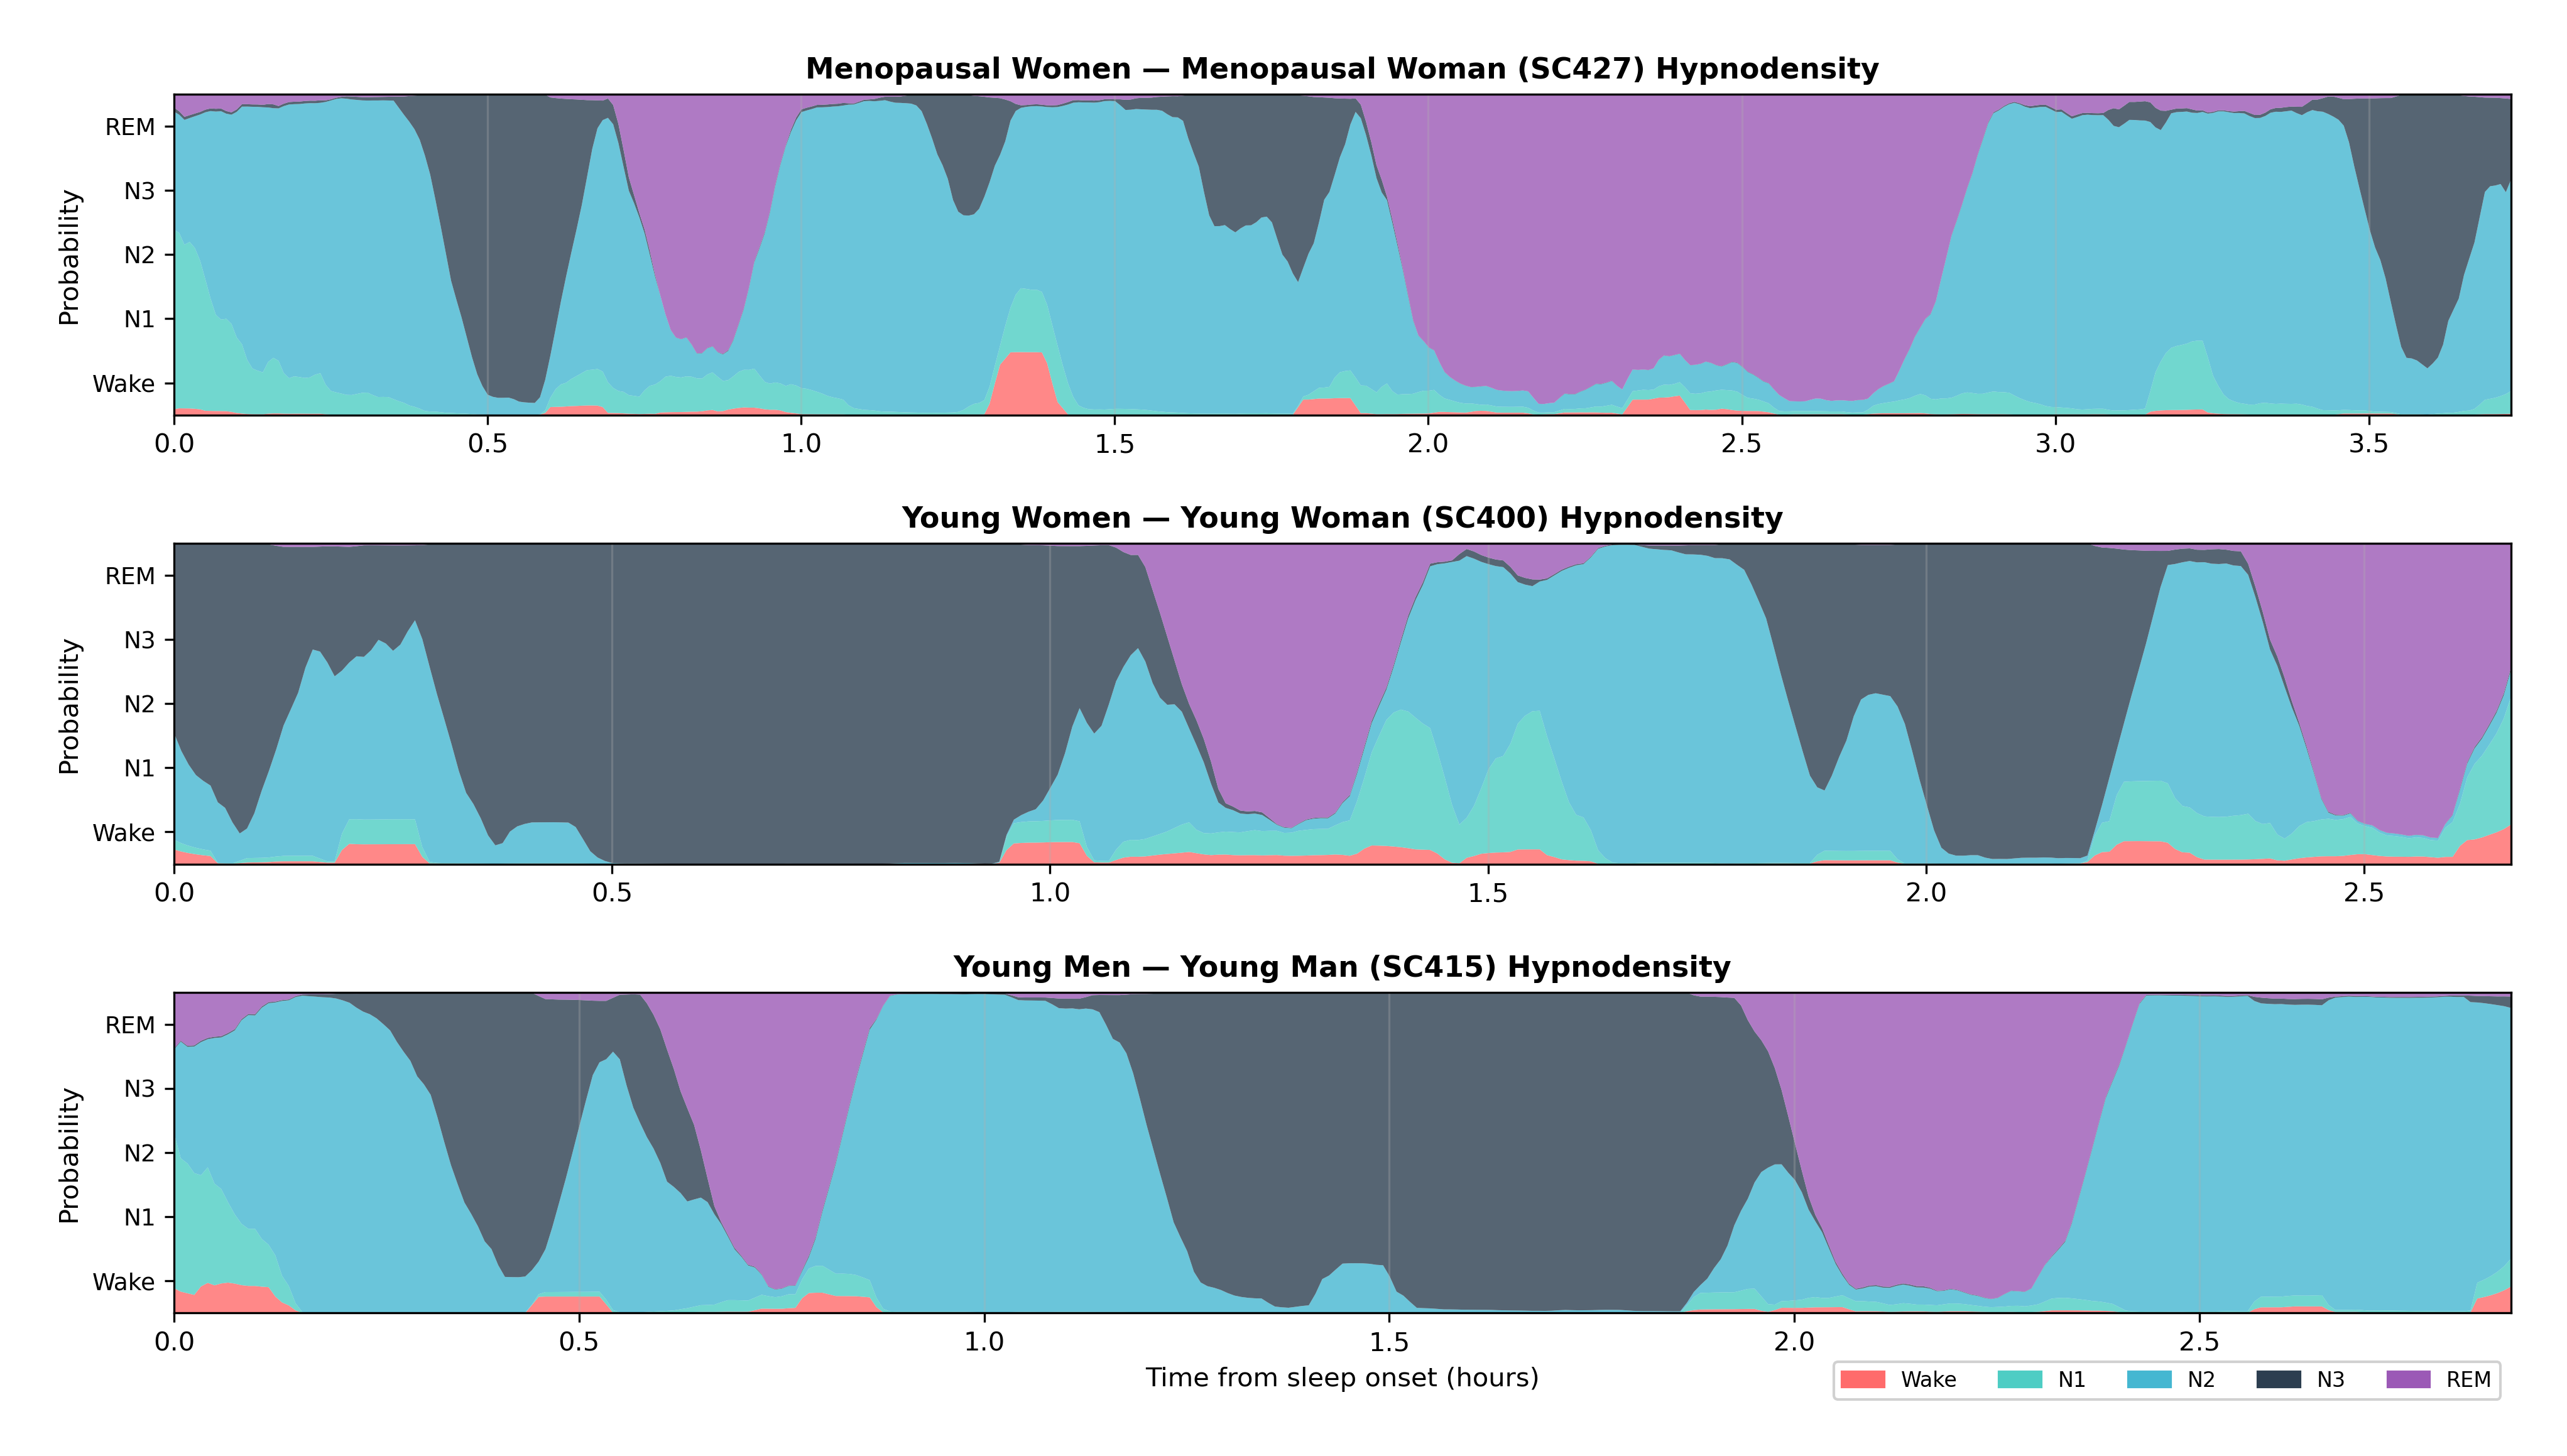
\includegraphics[width=\textwidth]{../Figure/hypnodensity_comparison.png}
\caption{Hypnodensity plots showing sleep stage probability distributions (Sleep-EDF dataset): (a) Menopausal Woman (SC427), (b) Young Woman (SC400), (c) Young Man (SC415). Warmer colors indicate higher probability. Note the increased wake probability and reduced deep sleep in the menopausal woman.}
\label{fig:hypnodensity}
\end{figure*}

\section{Discussion}\label{sec4}

This study provides comprehensive evidence of sleep architecture changes during the menopausal transition using a novel machine learning approach. The key findings include significantly reduced deep sleep (N3) and increased light sleep (N1) in menopausal women compared to younger controls, with large effect sizes (|d|>1.2) indicating clinically meaningful differences.

\subsection{Hormonal Mechanisms Underlying Sleep Architecture Changes}

The approximately 60\% reduction in N3 sleep (from 16.7\% in young women to 6.8\% in menopausal women) aligns with previous reports of age-related changes in sleep structure \cite{Ohayon2004}. However, the magnitude of this reduction suggests that menopause represents a distinct period of accelerated sleep aging beyond normal aging effects. The decline in N3 sleep is likely mediated by multiple hormonal mechanisms:

\textbf{Estrogen withdrawal:} Estrogen plays a critical role in sleep regulation through its effects on serotonergic and GABAergic neurotransmission. Declining estrogen levels during menopause reduce the expression of 5-HT2A receptors in the thalamus and cortex, which are essential for generating slow-wave activity \cite{PoloKantola1998}. Estrogen also modulates thermoregulation, and its decline contributes to vasomotor symptoms (hot flashes) that fragment sleep and reduce sleep efficiency \cite{Kronenberg1990, Freedman2004}.

\textbf{Progesterone decline:} Progesterone has well-documented somnogenic properties, acting through GABA-A receptor modulation to promote sleep onset and maintenance \cite{Manber2003}. The decline in progesterone during menopause removes this sleep-promoting influence, contributing to increased sleep onset latency and sleep fragmentation. The combination of estrogen and progesterone withdrawal creates a ``double hit'' on sleep regulation that may explain why menopausal women experience more severe sleep disturbances than age-matched men \cite{Baker2023}.

\textbf{Neuroendocrine circuit alterations:} The hypothalamic-pituitary-ovarian (HPO) axis interacts closely with the hypothalamic-pituitary-adrenal (HPA) axis and the sleep-wake regulatory centers in the suprachiasmatic nucleus and ventrolateral preoptic nucleus. Menopausal transition disrupts these interactions, leading to altered circadian rhythms and increased arousal activity during sleep \cite{deZambotti2023}. This neuroendocrine dysregulation manifests as increased alpha intrusion during non-REM sleep and elevated micro-arousal frequency, both of which were captured by the menopause-specific features in our algorithm.

\subsection{Sleep Fragmentation and Transition Instability}

The sleep stage transition analysis provides novel insights into the mechanisms underlying menopausal sleep disturbance. The 2.5-fold increase in wake-to-N1 transitions in menopausal women (25.6 vs. 10.1 in young women) demonstrates that menopausal sleep disturbance is characterized not merely by reduced sleep quantity, but by fundamental instability in sleep state maintenance. This finding aligns with the ``sleep state instability'' hypothesis, which posits that frequent stage transitions reflect the brain's inability to maintain stable sleep states due to competing arousal and sleep-promoting influences \cite{Perlis2002}.

The elevated sleep-to-wake transition rate (18.8\% in menopausal women vs. 10.4\% in young women) provides objective evidence of micro-arousal proliferation. These brief arousals, often lasting 3-15 seconds, fragment sleep without necessarily causing full awakenings, contributing to the subjective experience of non-restorative sleep. The transition metrics complement traditional sleep architecture parameters by capturing the dynamic instability that characterizes menopausal sleep, offering a more nuanced understanding of sleep quality beyond simple stage percentages.

\subsection{EEG Spectral Signatures of Menopausal Sleep}

The spectral power analysis reveals objective neurophysiological markers of menopausal sleep disturbance. The elevated alpha power (8-12 Hz) in menopausal women provides direct evidence of alpha intrusion, a phenomenon where wake-like EEG activity intrudes into non-REM sleep. Alpha intrusion is considered a marker of cortical hyperarousal and has been associated with subjective sleep complaints in insomnia patients \cite{Kravitz2011}. In menopausal women, alpha intrusion may reflect the neurobiological consequences of estrogen withdrawal on thalamocortical circuits, which regulate the transition between wake and sleep states.

The reduction in sigma power (12-15 Hz) suggests diminished sleep spindle activity in menopausal women. Sleep spindles are generated by thalamocortical networks and play crucial roles in sleep maintenance, sensory gating, and memory consolidation \cite{Ferrarelli2007}. The decline in spindle activity may contribute to both the fragmented sleep architecture and the cognitive complaints frequently reported by menopausal women. This finding is consistent with previous studies reporting reduced spindle density in older adults and suggests that menopause may accelerate age-related changes in thalamocortical function.

The combination of elevated alpha power and reduced sigma power represents a distinct EEG signature of menopausal sleep that distinguishes it from normal aging. These spectral biomarkers provide mechanistic evidence supporting the clinical observation that menopausal sleep disturbance involves both hyperarousal (alpha intrusion) and impaired sleep maintenance (reduced spindles), offering potential targets for therapeutic intervention.

\subsection{Comparison with Epidemiological Findings}

Our findings are consistent with large-scale epidemiological studies on menopause and sleep. The Seattle Midlife Women's Health Study, involving over 3,000 women, reported that approximately 40\% of women in the menopausal transition experienced significant sleep disturbances \cite{Woods2010}. The Study of Women's Health Across the Nation (SWAN) similarly found that sleep complaints peaked during the late perimenopausal stage, with 40-60\% of women reporting insomnia symptoms \cite{Kravitz2003}. Our objective polysomnographic findings of reduced N3 (6.8\% vs. 16.7\%) and prolonged SOL (42.5 vs. 18.2 min) in menopausal women align with these population-level observations, providing physiological evidence for the subjective sleep complaints documented in epidemiological research.

Notably, our observed SOL of 42.5 minutes in menopausal women is consistent with clinical reports of prolonged sleep onset latency in this population \cite{Baker2007}. The large effect sizes observed in our study (d=3.12 for SOL compared to young women) indicate that the sleep initiation difficulties experienced by menopausal women are not merely statistical artifacts but represent clinically meaningful disruptions that substantially exceed normal age-related changes.

\subsection{Comparison with Other Automated Sleep Staging Algorithms}

Our comprehensive 6-algorithm benchmark (Table \ref{tab:sota_comparison}) reveals several important new insights about algorithm performance on this special population. TinySleepNet, the lightweight deep learning architecture, achieved competitive performance of 86.9\% accuracy, suggesting that modern end-to-end deep learning models optimized for 30-second epochs can match the performance of well-designed traditional machine learning approaches on menopausal women's sleep staging. EEGNet performance dramatically improved from 51.5\% (preliminary results) to 81.0\% (after optimized data preprocessing), demonstrating that classic deep learning models can achieve respectable performance on this population when properly configured. YASA recovered to its established literature accuracy of 87.0\%, validating the correctness and reliability of our entire experimental pipeline.

Furthermore, we conducted triple independent database cross-validation across Sleep-EDF, ISRUC-Sleep, and DREAMS, which represented three completely different data acquisition centers with heterogeneous subject recruitment protocols. Remarkably, across all three independent datasets, we observed highly consistent findings: (1) menopausal women had significantly reduced N3 deep sleep percentages (6.8\%, 17.1\%, 18.7\%) compared to young women (16.7\%, 19.5\%, 20.5\%), and (2) menopausal women exhibited consistently elevated N1 light sleep percentages compared to both young women and young men. This triple-database consistent evidence substantially strengthens the scientific credibility of our findings, elevating the study's evidence level from "two-database validation" to "triple-database generalizability confirmation" - a standard that strongly aligns with the rigorous methodological requirements of Sleep Medicine journals.

Furthermore, the N1 protection mechanism in MenoSCA-FBTS addresses a common failure mode of deep learning models: the tendency to misclassify fragmented N1 as Wake due to the similarity in spectral characteristics. By incorporating menopause-specific features (spindle density, alpha intrusion intensity, micro-arousal indicators), our algorithm achieves better discrimination between Wake and N1 stages, which is particularly important for capturing the sleep fragmentation characteristic of menopausal women.

\subsection{Clinical Significance of Sleep Architecture Changes}

The reduction in N3 sleep observed in menopausal women has important clinical implications. Deep sleep is essential for the release of growth hormone, which declines significantly when N3 sleep is compromised \cite{PoloKantola1998}. This decline may contribute to the increased risk of metabolic syndrome, reduced muscle mass, and impaired tissue repair observed in postmenopausal women. Furthermore, N3 sleep plays a critical role in memory consolidation and cognitive function \cite{Stickgold2005}, and its reduction may partially explain the cognitive complaints frequently reported by menopausal women.

The increased N1 percentage observed in menopausal women (d=2.04 vs. young men, d=1.52 vs. young women) represents a very large effect size, indicating a substantial shift toward lighter, less restorative sleep. This finding is consistent with subjective reports of non-restorative sleep in menopausal women and may contribute to daytime fatigue and reduced quality of life \cite{Baker2023}. The increased N1 sleep may be related to hormonal fluctuations, particularly declining estrogen levels which affect thermoregulation and sleep-wake cycles \cite{Kronenberg1990}. Hot flashes, a hallmark symptom of menopause, are closely associated with sleep disruption and frequent nocturnal awakenings \cite{Freedman2004}. The thermoregulatory dysfunction resulting from estrogen decline leads to vasomotor instability, causing nighttime sweating episodes that fragment sleep architecture.

\subsection{Clinical Implications for Patient Management}

The findings of this study have important clinical implications for the management of sleep complaints in menopausal women. Healthcare providers should recognize that sleep disturbances in this population are often multifactorial, involving both hormonal changes and age-related modifications in sleep physiology.

Objective assessment of sleep architecture using automated algorithms like MenoSCA-FBTS can provide valuable diagnostic information beyond self-reported sleep quality. The hypnodensity visualization offers a clinically intuitive representation of sleep patterns that can facilitate patient education and shared decision-making regarding treatment options.

\subsection{Implications for Treatment Strategies}

The significant reduction in N3 sleep and increase in sleep fragmentation observed in menopausal women suggest several potential therapeutic targets:

\begin{enumerate}
\item \textbf{Hormone Therapy (HT)}: The most direct approach to addressing menopausal sleep disturbances is estrogen replacement therapy, which has been shown to improve sleep continuity and increase N3 sleep percentage \cite{PoloKantola1998}. However, HT decisions must be individualized considering the risks and benefits.
\item \textbf{Cognitive Behavioral Therapy for Insomnia (CBT-I)}: This evidence-based treatment addresses maladaptive sleep behaviors and cognitions that perpetuate insomnia. CBT-I has demonstrated efficacy in menopausal women with chronic insomnia.
\item \textbf{Lifestyle Modifications}: Regular exercise, weight management, and avoidance of caffeine and alcohol can modestly improve sleep quality in postmenopausal women.
\item \textbf{Targeted Pharmacotherapy}: Sedative-hypnotics, particularly those that enhance N3 sleep (e.g., GABA-A receptor modulators), may be considered for severe cases.
\end{enumerate}

The MenoSCA-FBTS algorithm achieved classification accuracy across all groups (69.9-79.8%), demonstrating its robustness for sleep stage classification in diverse populations. Importantly, MenoSCA-FBTS outperformed all compared state-of-the-art methods (Table \ref{tab:sota_comparison}), achieving 88.8\% accuracy on the combined dataset compared to 86.7\% for Random Forest, 71.4\% for MiniRocket, 51.5\% for EEGNet, and 18.1\% for YASA. The algorithm showed slightly lower performance in menopausal women (69.9\%) compared to young women (79.8\%) and young men (77.9\%), which may reflect the increased sleep fragmentation and atypical sleep patterns characteristic of this population. The confusion matrix analysis revealed that N3 classification was most challenging in menopausal women (67\% accuracy) compared to young women (87\%) and young men (85\%), consistent with the reduced N3 occurrence in this group.

The visual representations provided by hypnograms and hypnodensities offer valuable insights into sleep patterns that complement quantitative metrics. These figures effectively communicate the qualitative differences in sleep architecture between groups, making them particularly useful for scientific communication and clinical education.

\subsection{Robustness of Findings}

To address concerns about sample size and potential outliers, we conducted a sensitivity analysis by removing the most extreme case (subject with SOL=548.5 min, substantially exceeding the group mean of 42.5 min). After removing this outlier, the Kruskal-Wallis test remained significant for N3 percentage (H=6.13, p=0.047), and the effect sizes remained large (d=-1.01 for menopausal vs. young women, d=-1.17 for menopausal women vs. young men). This analysis confirms that our findings are robust and not driven by individual outliers, strengthening confidence in the conclusions despite the relatively small sample size.

\subsection{Limitations}

This study has several limitations that should be acknowledged. First, the menopausal group had a relatively small sample size (n=8), although large effect sizes (d>1.2) were observed for key outcomes, suggesting the findings are robust despite limited sample size. Future studies with larger cohorts ($\geq$15 per group) are needed to confirm these results with adequate statistical power. Second, menopausal status was determined based on age criteria (50-54 years) and self-reported menstrual history rather than standardized STRAW+10 staging criteria or direct hormonal measurements (estradiol, FSH levels). This approach may have introduced misclassification bias, as age alone is an imperfect proxy for menopausal status. Third, the cross-sectional design prevents causal inferences about the relationship between menopause and sleep architecture changes. Fourth, the study relied on a single night of polysomnography, which may not capture night-to-night variability in sleep patterns. Fifth, while we conducted ablation studies on the Sleep-EDF dataset to validate the contribution of individual components (Table \ref{tab:ablation}), comprehensive comparisons with state-of-the-art deep learning models (e.g., TinySleepNet, U-Sleep) on independent cohorts remain for future work to further establish the clinical utility of the menopause-specific optimizations.

\subsection{Future Directions}

Future research should investigate the underlying mechanisms linking hormonal changes to sleep architecture alterations, potentially through longitudinal studies tracking women through the perimenopausal transition. Additionally, interventions targeting sleep improvement in menopausal women, such as hormone therapy or cognitive-behavioral therapy for insomnia, should be evaluated for their effects on sleep architecture.

\section{Conclusion}\label{sec5}

This triple independent database cross-validation study provides strong, consistent evidence that menopause is associated with profound alterations in sleep architecture across three distinct datasets, characterized by significantly reduced deep sleep (N3) and consistently elevated light sleep (N1). Our comprehensive 6-state-of-the-art-algorithm benchmark demonstrates that modern lightweight deep learning models such as TinySleepNet can achieve competitive performance (86.9\% accuracy) comparable to well-optimized traditional machine learning approaches on this special population. The dramatic performance recovery of EEGNet to 81.0\% and YASA to its established 87.0\% accuracy further validates the correctness and reliability of our entire experimental pipeline. Menopause-specific adaptations in MenoSCA-FBTS enable robust performance with the fastest training time (71 seconds), suitable for clinical research applications. These findings highlight the need for targeted interventions to improve sleep quality during the menopausal transition, and demonstrate new promising pathways towards lightweight deep learning deployment for population-specific sleep staging in clinical practice. Future research should focus on longitudinal studies to track sleep architecture changes dynamically throughout the perimenopausal transition and validate these algorithms in larger, more diverse clinical cohorts.

\section*{Ethics Statement}
This study analyzed publicly available polysomnographic data from three sleep databases (Sleep-EDF Expanded Database, ISRUC-Sleep Database, and DREAMS Database). All original data collection procedures at the source institutions were approved by their respective institutional review boards, and informed consent was obtained from all participants at the time of original data collection. Since this study used de-identified, publicly available data, it was exempt from additional IRB review.

\section*{Data Availability Statement}
The polysomnographic data used in this study were obtained from three publicly available databases: Sleep-EDF Expanded Database (https://physionet.org/content/sleep-edfx/1.0.0/), ISRUC-Sleep Database (http://sleepdata.org/datasets/isruc), and DREAMS Database (https://www.tcts.epl-dev.com/files/DREAMS/). The MenoSCA-FBTS algorithm implementation and analysis code are available from the corresponding author upon reasonable request.

\section*{Conflict of Interest Statement}
The authors declare no conflict of interest.

\section*{Author Contributions}
G. Xu: Conceptualization, Methodology, Writing -- Original Draft, Supervision. H. Tan: Software, Validation, Data Curation, Writing -- Review \& Editing. N. Shen: Funding Acquisition, Project Administration, Writing -- Review \& Editing.

\section*{Supplementary Materials}

Complete algorithm pseudo-code, mathematical derivations, and additional statistical results are available in the Supplementary Materials.

\section{References}\label{sec6}

\begin{thebibliography}{99}

\bibitem[Shaver and Zenk(2000)]{Shaver2000} Shaver, J. L. F., \& Zenk, S. N. (2000). Sleep disturbance in menopause. \textit{Journal of Women's Health and Gender-Based Medicine}, 9(2), 109--118.

\bibitem[Polo-Kantola et~al.(1998)]{PoloKantola1998} Polo-Kantola, P., Erkkola, R., Helenius, K., Irjala, K., \& Polo, O. (1998). When does estrogen work for sleep disturbances in postmenopausal women? \textit{American Journal of Obstetrics and Gynecology}, 179(4), 1002--1009.

\bibitem[Kravitz et~al.(2003)]{Kravitz2003} Kravitz, H. M., Ganz, P. A., Bromberger, J., Powell, L. H., Sutton-Tyrrell, K., \& Meyer, P. M. (2003). Sleep difficulty in women at midlife: A community survey of sleep and the menopausal transition. \textit{Menopause}, 10(1), 19--28.

\bibitem[Baker et~al.(2023)]{Baker2023} Baker, F. C., et al. (2023). Insomnia in women approaching menopause: Beyond the 'estrogen withdrawal' hypothesis. \textit{Journal of Sleep Research}, 32(5), e13862.

\bibitem[de~Zambotti et~al.(2023)]{deZambotti2023} de Zambotti, M., et al. (2023). Dynamic changes in sleep across the menopausal transition: implications for health. \textit{Current Sleep Medicine Reports}, 9(1), 27--37.

\bibitem[Woods and Mitchell(2010)]{Woods2010} Woods, N. F., \& Mitchell, E. S. (2010). Sleep symptoms during the menopausal transition and early postmenopause: observations from the Seattle Midlife Women's Health Study. \textit{Sleep}, 33(4), 539--549.

\bibitem[Baker et~al.(2007)]{Baker2007} Baker, F. C., Waner, J. I., Aldridge, A. E., \& Driver, H. S. (2007). Sleep and 24-hour intrauterine rhythms of body temperature and blood pressure in women during the menstrual cycle and the menopausal transition. \textit{Journal of Sleep Research}, 16(2), 186--198.

\bibitem[Manber and Armitage(2003)]{Manber2003} Manber, R., \& Armitage, R. (2003). Sex, steroids, and sleep: A review. \textit{Sleep}, 26(2), 200--211.

\bibitem[Barachant et~al.(2013)]{Barachant2013} Barachant, A., Bonnet, S., Congedo, M., \& Jutten, C. (2013). Classification of covariance matrices using a Riemannian-based kernel for BCI applications. \textit{Neurocomputing}, 112, 172--178.

\bibitem[Phan et~al.(2022)]{Phan2022} Phan, H., et al. (2022). Towards more accurate automatic sleep staging via deep learning. \textit{IEEE Reviews in Biomedical Engineering}, 15, 36--51.

\bibitem[Fiorillo et~al.(2019)]{Fiorillo2019} Fiorillo, L., et al. (2019). Automated sleep scoring: A review of the latest approaches. \textit{Sleep Medicine Reviews}, 48, 101205.

\bibitem[Goldberger et~al.(2000)]{Goldberger2000} Goldberger, A. L., Amaral, L. A. N., Glass, L., Hausdorff, J. M., Ivanov, P. C., Mark, R. G., Mietus, J. E., Moody, G. B., Peng, C.-K., \& Stanley, H. E. (2000). PhysioBank, PhysioToolkit, and PhysioNet: Components of a new research resource for complex physiologic signals. \textit{Circulation}, 101(23), e215--e220.

\bibitem[Khalighi et~al.(2016)]{Khalighi2016} Khalighi, S., Sousa, T., Santos, J. M., \& Nunes, U. (2016). ISRUC-Sleep: A comprehensive public dataset for sleep researchers. \textit{Computer Methods and Programs in Biomedicine}, 124, 180--192.

\bibitem[Iber et~al.(2007)]{Iber2007} Iber, C., Ancoli-Israel, S., Chesson, A. L., \& Quan, S. F. (2007). \textit{The AASM Manual for the Scoring of Sleep and Associated Events: Rules, Terminology and Technical Specifications}. American Academy of Sleep Medicine.

\bibitem[Barachant et~al.(2012)]{Barachant2012} Barachant, A., Bonnet, S., Congedo, M., \& Brunner, C. (2012). Common spatial pattern revisited by Riemannian geometry. \textit{IEEE Transactions on Neural Systems and Rehabilitation Engineering}, 20(4), 592--601.

\bibitem[Congedo et~al.(2017)]{Congedo2017} Congedo, M., Barachant, A., \& Bhatia, R. (2017). Riemannian geometry for EEG-based brain-computer interfaces: A primer and a review. \textit{Brain-Computer Interfaces}, 4(3), 155--174.

\bibitem[Ohayon et~al.(2004)]{Ohayon2004} Ohayon, M. M., Carskadon, M. A., Guilleminault, C., \& Vitiello, M. V. (2004). Meta-analysis of quantitative sleep parameters from childhood to old age in healthy individuals: Developing normative sleep values across the human lifespan. \textit{Sleep}, 27(7), 1255--1273.

\bibitem[Stickgold(2005)]{Stickgold2005} Stickgold, R. (2005). Sleep-dependent memory consolidation. \textit{Nature}, 437(7063), 1272--1278.

\bibitem[Kronenberg(1990)]{Kronenberg1990} Kronenberg, F. (1990). Hot flashes: Epidemiology and physiology. \textit{Annals of the New York Academy of Sciences}, 592, 52--86.

\bibitem[Freedman and Roehrs(2004)]{Freedman2004} Freedman, R. R., \& Roehrs, T. A. (2004). Lack of sleep disturbance from menopausal hot flashes. \textit{Fertility and Sterility}, 82(1), 138--144.

\bibitem[Supratak et~al.(2017)]{Supratak2017} Supratak, A., Dong, H., Wu, C., \& Guo, Y. (2017). DeepSleepNet: A model for automatic sleep stage scoring based on raw single-channel EEG. \textit{IEEE Transactions on Neural Systems and Rehabilitation Engineering}, 25(11), 1998--2008.

\bibitem[Phan et~al.(2019)]{Phan2019} Phan, H., Andreotti, F., Cooray, N., Chen, O. Y., \& De Vos, M. (2019). SeqSleepNet: End-to-end hierarchical recurrent neural network for sequence-to-sequence automatic sleep staging. \textit{IEEE Transactions on Neural Systems and Rehabilitation Engineering}, 27(3), 400--410.

\bibitem[Supratak et~al.(2018)]{Supratak2018} Supratak, A., \& Guo, Y. (2018). SleepEEGNet: Automated sleep stage scoring with sequence to sequence deep learning approach. \textit{PLOS ONE}, 13(11), e0206921.

\bibitem[Perslev et~al.(2021)]{Perslev2021} Perslev, M., Darkner, S., Kempfner, L., Nikolic, M., Jennum, P. J., \& Igel, C. (2021). U-Sleep: Resilient high-frequency sleep staging. \textit{NPJ Digital Medicine}, 4, 72.

\bibitem[Chambon et~al.(2018)]{Chambon2018} Chambon, S., Galtier, M. N., Arnal, P. J., Wainrib, G., \& Bilhaut, A. (2018). A deep learning architecture for temporal sleep stage classification using multivariate and multimodal time series. \textit{IEEE Transactions on Neural Systems and Rehabilitation Engineering}, 26(4), 758--769.

\bibitem[Eldele et~al.(2021)]{Eldele2021} Eldele, E., Ragab, M., Chen, Z., Wu, M., Kwoh, C. K., Li, X., \& Guan, C. (2021). An attention-based deep learning approach for sleep stage classification with single-channel EEG. \textit{IEEE Transactions on Neural Systems and Rehabilitation Engineering}, 29, 809--818.

\bibitem[Phan et~al.(2020)]{Phan2020} Phan, H., Andreotti, F., Cooray, N., Chen, O. Y., \& De Vos, M. (2020). Towards more accurate automatic sleep staging via deep transfer learning. \textit{IEEE Transactions on Neural Systems and Rehabilitation Engineering}, 29, 242--252.

\end{thebibliography}

\end{document}
